
    XXX muss vmtl eig in BAsics
    To evaluate the quality of the material parameters we need a possibility to investigate the material response caused by the definition of the material parameters. Then we can compare this results with the load parameters and evaluate the quality of the current material parameters. Thus we have to use a simulation program to analyse the material behaviour for every iteration of material parameter values during the optimization process. We decided to use ABAQUS as simulation software, because of the intern scripting tool. With the ABAQUS scripting tool one can run python scripts directly in ABAQUS (see chapter XX). With special ABAQUS commands one can use ABAQUS with the same opportunities as with the GUI. 
    XXXX

    Therefore we choose simple load cases, which are easy to recalculate. AS explained in the chpater XX about the mathematical problem formulation, we have to define a parameter which defines the quality of the mechanical responses calculated by ABAQUS compared to the ones from the MD-simulation. Therefore we first have to define adequate mechanical measurements which represent best the mechanical behaviour and contain information about the material parameters. Hence the stress and strain measurements in all normal and shear directions are possible quantities. Depending on the load case the measurements with the most useful information may vary.
    

    
    \chapter{Models and Methods}

    In the following chapter we describe the optimisation process used in this thesis. Therefore we first have a closer look on the theoretical structure of the process. Afterwards we discuss the implementation with all 

    \section{Theory}

    The aim of the optimisation process is to find material parameters which best represent the mechanical behaviour analysed with a MD-Simulation. In the following we demonstrate the need of this process.
    The MD-analysis gives information about the mechanical response for an applied load case. In a MD-simulation we can apply a load case and log the stress and strain values in all directions at prescribed time steps during the loading process. In the following this data from the MD-Simulations are called load parameters. They describe the applied load (for example uniform strain up to 20\(\%\)) and the corresponding reactions. In \autoref{subsec:loadParameters} we have a closer look on the structure of the data. 
    This load parameters empirically describe the mechanical behaviour of the investigated material. However, we are interested in a deterministic description of the material behaviour. This is usually done by the definition of material parameters. Since it is not possible to specify material parameters directly in the MD-simulation, we want to build a optimization process which is able to find the best material parameters to represent the material behaviour from the load parameters. To implement this problem we have to reformulate it as a minimization problem. As minimization value we have to define a value that represents the error of mechanical response of the material. Therefore we compare the material behaviour defined through the material parameters with the one from the load parameters. If we minimise their difference, we improve the quality of the material parameter values describing the material behaviour. In our problem formulation we have now the optimisation of the material parameters controlled by the minimization of the difference between the mechanical responses. In the next step we need to define this difference between the mechanical behaviour more precisely. For the mathematical formulation only one single value is allowed for the problem formulation. For a detailed explanation we now introduce the used model, the load cases and load parameters.

    As explained in chapter XX we use ABAQUS as simulation software and the ABAQUS internal scripting tool for the code. 
    
    
    \section{Model, load cases and load parameters}
    In this section we introduce the used model and the applied load cases. 
    As model we use a simple isotropic cube of size 1x1x1. We use it as one representative part of an infinitely extended material which is modelled through easyPBC (see chapter xx section XX). By the usage of this simple geometry we anticipate short simulation times. During the optimization process this property is important for a fast evaluation of the result quality. In addition the mechanical responses of a cube are comprehensible and it is possible to verify the results by hand computations. However, it is easy to apply different load cases on a cube. As we see in chapter XX, we have to modify the load applied by easyPBC. This is much easier at a simple geometry where we can apply uniform stresses or strains. Then it is simple to check the correctness of the load application since qualitative the mechanical responses for these load cases are known. (BEISPIEL BILD MIT LOAD CASE)
    
    NOCH MEHR ÜBER DAS MODEL
    
    \subsection{Load cases and evaluation measurements}\label{subsec: loadCases}
    
    A load case defines the direction where the load is applied. Since we want reproducible and easy cases, we only allow loading in normal directions and principal shear directions. To aplly this loadings we use easyPBC. For a consistent naming, we adopt the naming from easyPBC for the load cases, which is defined in \autoref{tab:loadCaseNaming}.
     To model a more complex loading situation it is possible to combine these load cases. For example it is possible to apply a tensile load in xx-direction combined with a shear strain in xz-direction. Important to notice is, that we apply load only in one direction per load case without constraining the other ones. Thus the deformation of the cube is only restricted through the periodic boundary conditions (see chapter XX) which ensure that parallel surfaces remain parallel during the deformation process. Apart from this, the material response is not restricted. After the application of a load case, we have to decide which material responses we use to compare with our load parameters. We have the possibility to read out the stress and strain values in all normal and shear directions. These values are called evaluation measurements. For a high result quality of our material parameters, we try to use evaluation measurements where we can extract the most information about our material behaviour. These measurements vary depending on the applied load case. As we see in section XX the user defines the evaluation measurements in the input file. Based on the presented load cases in the following, the meaning of the evaluation measurements becomes clear. 

    \begin{table}[H]
        \centering
        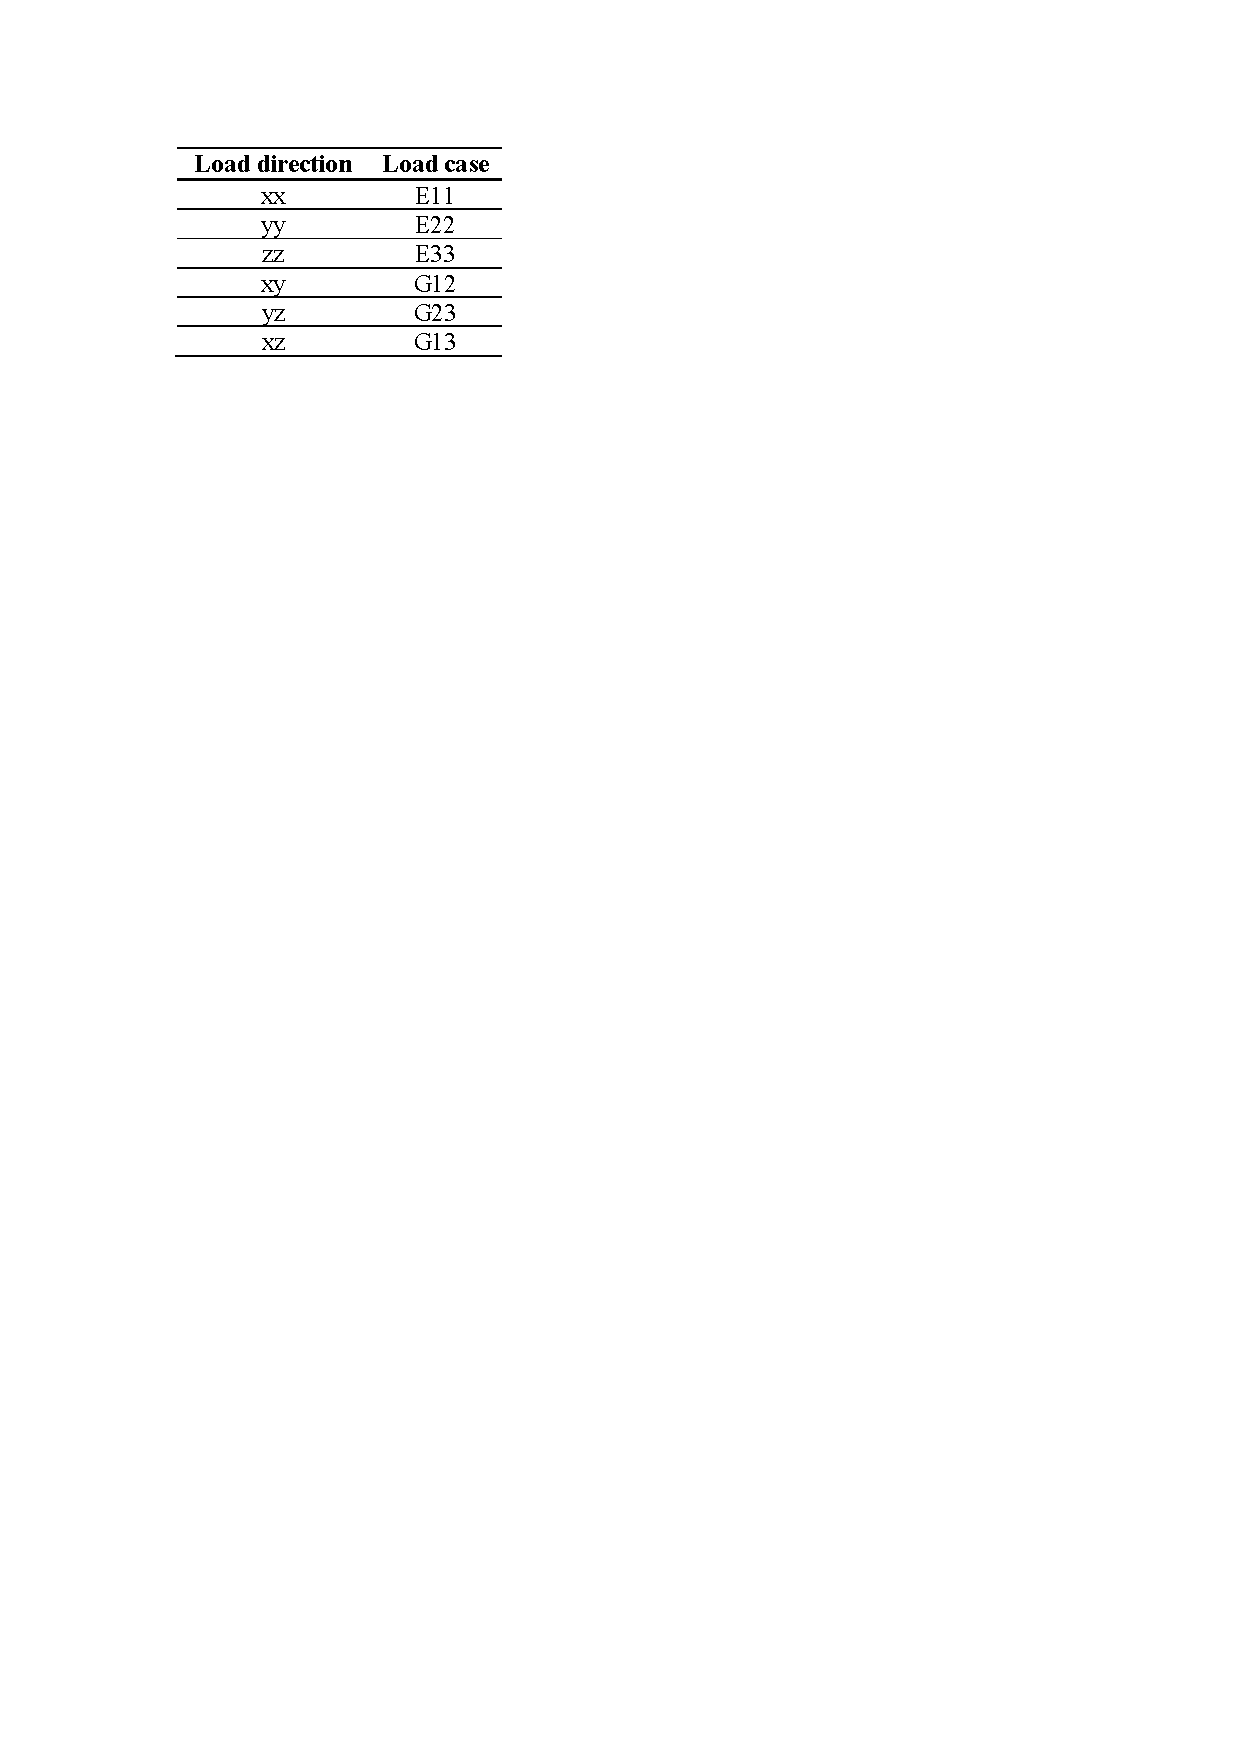
\includegraphics[width=0.35\textwidth]{loadCaseNaming.pdf}
		\caption{Load case naming}
		\label{tab:loadCaseNaming}
    \end{table}

    For the verification of the code we use a simple tensile load case E11.
    In all other directions we do not apply any constraints except the periodic boundary conditions. As evaluation measurements we use the stress in x-direction and the lateral strains in normal y- and z-direction. The normal stress in x-direction contains information about the Young's modulus and the plastic parameters. For the Poisson ratio the lateral strains are necessary. Since we do not constrain the motion of the cube, the y- and z-dimension will decrease, to balance the strain in x-direction. This reaction is necessary to keep a state of minimum stress. Simultaneously this means that the lateral stresses do not contain any useful information in this load case, because they are numerically zero. 
    The validation study is done with the same load case. Similar to the verification study we need the stresses in x-direction and the lateral strains to extract information about all material parameters. 
    In the next step we use a load case E11, then G12 and finally combine them. Through the additional obtained information we try to improve the uniqueness of the determined material parameter values. As evaluation measurement for the load case G12 we use the stresses in this direction.
    As a last study we investigate the application of cyclic loading as E11 load case. We perform this study with varying load parameters (see \autoref{subsec:loadParameters}). 


    \begin{figure}
		\centering
        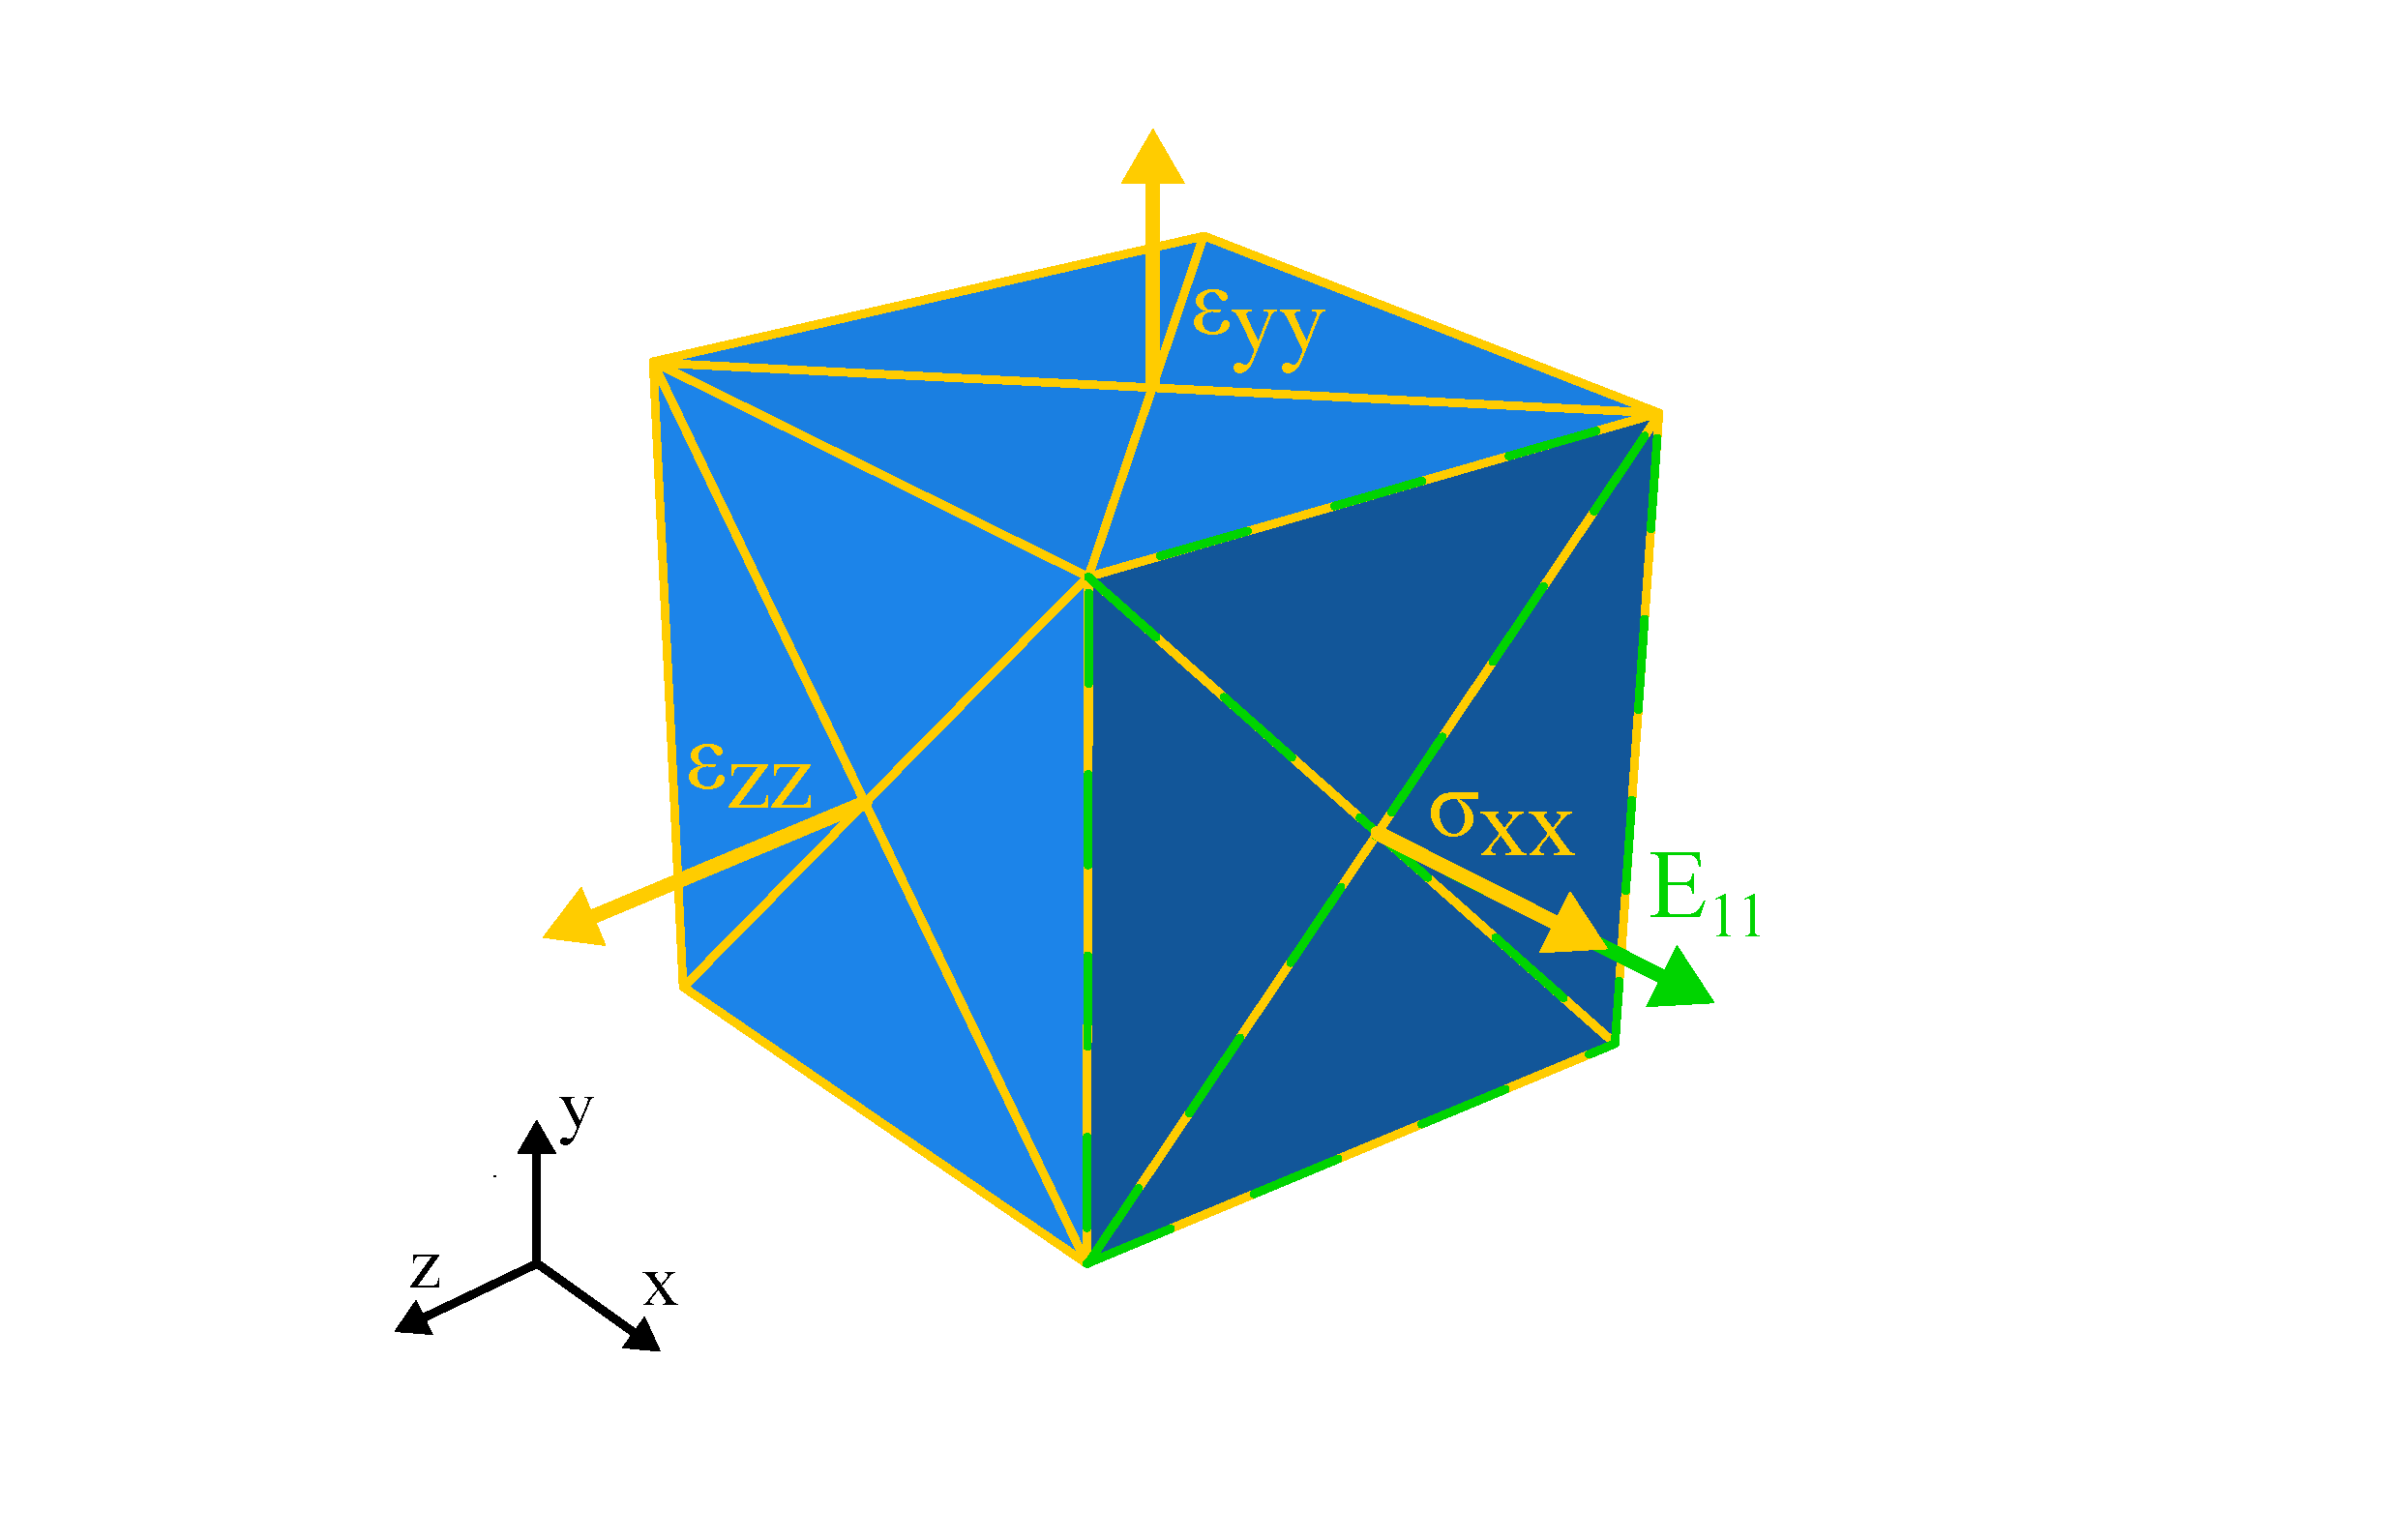
\includegraphics[width=0.7\textwidth]{cube_loading_plain_white_new.pdf}
		\caption{illustration of load case and evaluation measurements}
		\label{fig:loadCaseEvaluationMeasurements}
	\end{figure}

    \subsection{Load parameters}\label{subsec:loadParameters}
    The load parameters contain the stress and strain values measured during the MD-simulation. The values are stored for all normal and shear directions. From this file we can extract the quantitave values of the applied load. Since we defined the load cases similar to the ones in the MD-simulations, we can use the data directly. They contain stress and strain values for every MD-timestep. The meaning of the MD-timsteps is not relevant in this thesis, because it depends on several restrictions on the MD-simulation which will not be discussed in this context. Within in the scope of this work it is only important that we get stress and strain values for multiple steps during the loading process. Thus, we can register different trends of loading and the corresponding responses. If we know the load case, we can easily extract the corresponding loading parameters and transfer them into the ABAQUS model. A detailed description of the of the load application in ABAQUS can be found in \autoref{sec: preprocessing}. Besides, we need some stress or strain values which define the material responses in the MD-simulation to evaluate the material parameter fitting. The introduced evaluation measurements \autoref{subsec: loadCases} define which data from the load parameters are used for the optimization process. In XX the load cases and load parameters we investigate in this work are shown.
    In the verification and validation studies we always apply a linear strain with a maximum value of 20\%. In the validation studies we use different mixing ratios as materials which show different mechanical behaviours. In the next study we investigate a tensile strain following a sinus function over time with a maximum amplitude of 15 \(\%\) strain. We only consider the first quarter of a period up to the maximum value as a preparation for studies with cyclic loading. In this preparing study we want to investigate the handling with non-linear loadings. Then we use the same load parameters but apply them as a shear strain. In the next step we use the same load parameters but combine the load cases of E11 and G12. Important to notice is that the previously introduced load parameters proceed in a wide strain range. Assuming that the material starts to palstify at XX, the majority of the loaing steps are located in the plastic domain of the material. Conversely, the load parameters contain only little information about the elastic material behaviour. In \autoref{sec: verification} the issue about this unequal distribution in the material domains becomes clear.    
    As a last study we investigate  a full period of a sinusoidal loading for a tensile load case in x-direction. We use amplitudes of 1\(\%\), 5\(\%\) and 8\(\%\). Through the use of this load parameters we try to get a larger proportion of data points in the elastic domain.

    \begin{table}[H]
        \centering
        \renewcommand{\arraystretch}{1.3}
        \caption{Overview of test series, load cases and load parameters.}
        \begin{tabular}{L{0.15\textwidth}C{0.06\textwidth}C{0.13\textwidth}C{0.13\textwidth}C{0.1\textwidth}C{0.2\textwidth}}
        \toprule
        \multirow{3}{0.15\textwidth}{\textbf{Test series}} & \multirow{3}{0.06\textwidth}{\textbf{Load case}} & \multicolumn{3}{C{0.36\textwidth}}{\textbf{Load parameters}} & \multirow{3}{0.2\textwidth}{\textbf{Evaluation measurements}}\\  \cmidrule{3-5}
        & & \multirow{2}{0.13\textwidth}{\textbf{Trajectory}} & \multirow{2}{0.13\textwidth}{\textbf{Amplitude}} &  \multirow{2}{0.1\textwidth}{\textbf{Mixing ratio}} \\ 
         &&&&&\\ \midrule
        Verification & E11 & Linear & 20\% & 6:3 & \(\sigma_{xx}, \varepsilon_{yy}, \varepsilon_{zz}\)\\\hline
        Validation & E11 & Linear & 20\% & 4:3 & \(\sigma_{xx}, \varepsilon_{yy}, \varepsilon_{zz}\)\\ 
                &     &        &      & 6:3 \\ 
                &     &        &      & 8:3 \\ \hline
        \multirow{2}{0.15\textwidth}{Normal strain} & E11 & Sinus (\(\frac{1}{2} \pi\)) & 15\% & 6:3 & \(\sigma_{xx}, \varepsilon_{yy}, \varepsilon_{zz}\)\\ 
                &   &           &   && \\ \hline
        Shear strain  & E11 & Sinus (\(\frac{1}{2}\pi\)) & 15\% & 6:3 & \(\sigma_{xy}\)\\ \hline
        \multirow{2}{0.15\textwidth}{Normal \& Shear strain} & E11 & Sinus (\(\frac{1}{2}\pi\)) & 15\% & 6:3 & \(\sigma_{xx}, \varepsilon_{yy}, \varepsilon_{zz}, \sigma_{xy}\)\\ 
                                & G12 &       &      &     \\ \hline
        \multirow{2}{0.15\textwidth}{Normal strain} & E11 & Sinus (\(2\pi\)) & 1\%  & 6:3 & \(\sigma_{xx}, \varepsilon_{yy}, \varepsilon_{zz}\)\\ 
                    &     &       & 5\%  & 6:3 & \(\sigma_{xx}, \varepsilon_{yy}, \varepsilon_{zz}\)\\ 
                    &     &       & 8\%  & 6:3 & \(\sigma_{xx}, \varepsilon_{yy}, \varepsilon_{zz}\)\\ \bottomrule
        \end{tabular}
        
    \end{table}



    \subsection{Error calculation}\label{subsec: errorCalculation}
    The stress and strain measurements we do for the introduced load cases need to be reduced to one single value per load case for the mathematical solution of the optimization problem. 
    In this section we explain how we do this reduction. 
    First we define the measurements we want to use in the current load case. Then we read out this measurements from the ABAQUS-analysis and from the MD-analysis. In the next step we have to build the difference between them. For the tensile load case for example we have to do this for multiple measurements (stress xx, strain yy, strain zz). Additional it is not enough to consider only the stress and strain values at the end of the applied load (at 20 percent). If we want to adequately describe the material behaviour it is sufficient to regard the measurement during the complete loading process. From the MD-simulation certain strain-values are given at which stresses and strain in other directions are measured. We use this strain-values as steps in the ABAQUS-simulation to read the measurements there too. Thus we are able to directly compare the evolution of the measurements during the loading process. Since we now have multiple measurements to evaluate for multiple strain steps we need a mathematical expression to reduce all this values into one. For a representative value we decide to build a root-mean-squared error (RMSE). NOCH MEHR DAZU THEORIE. 
    TO build this value we first compute the squared difference between the ABAQUS measurement value and the MD measurement value at every strain step for all necessary measurements. The result is one array with squared differences for every measurement quantity used in the load case. As described in chapter XX the distribution of the data points is unfavourable for the determination of the elastic parameters because only one data point is included in the elastic domain of the material. To support the algorithm to find the elastic parameters anyway we applied a weight of 100 at the data point in the elastic domain for every measurement quantity. In the next step we build the mean value out of the weighted arrays separate for every measurement quantity. Now we have mean squared errors for all measurements of the current load case. If we now build one value out of this mean squared errors we have to ensure a common scale of the values. Otherwise their influence on the overall error may vary significantly. Therefore it is necessary to apply weights to the mean squared errors of certain measurement quantities. The exact weights depend on the load case and the used data set. In general, the mean squared errors of strain measurements are much smaller than the ones from stress measurements, such that a weight of around 10e4 is necessary for the strain measurements. After that we sum up the weighted mean squared errors and build again a mean value. From this value we build then the square root. Since our code is able to process multiple load cases for one data set in one optimisation process we can calculate the RMSE for every load case and apply weights depending on the load case. Then we sum up all these weighted RMSE values and use it as return value for our minimization function. Additional, multiple data sets can be processed which leads to a repetition of the described procedure for every data set. Therefore we can calculate the return value for multiple load cases for multiple data sets. Then we can apply weights for every data set and sum it again to return a single value. This value is the value we return our minimization function. Through the adaption of the material values this value should be minimized. \\
    IN the following sections we have a closer look on the implementation of this minimization process. 
    \begin{center}
        \begin{gather}
            \text{mse}_{\sigma} = \frac{\displaystyle\sum_{i=1}^{N_\text{frame}} w_i (\sigma_{odb,i} - \sigma_{md,i})^2}{\displaystyle\sum_{i=1}^{N_\text{frame}}w_i } 
            \hspace{2cm}
            \text{mse}_{\varepsilon} = \frac{\displaystyle\sum_{i=1}^{N_{\text{frame}}} w_i (\varepsilon_{odb,i} - \varepsilon_{md,i})^2}{\displaystyle\sum_{i=1}^{N_\text{frame}}w_i } \\
            \text{rmse} = \sqrt{\frac{\displaystyle\sum_{j=xx}^{N_\text{SED}} w_{\sigma} \cdot \text{mse}_{\sigma,j} + \displaystyle\sum_{j=1}^{N_\text{EED}} w_{\varepsilon} \cdot \text{mse}_{\varepsilon,j}}{N_\text{SED} + N_\text{EED}}} \\
            \text{error} = \sum_{k=1}^{N_\text{LC}} \sum_{l=1}^{N_\text{LP}} w_k w_l \cdot \text{rmse}_{k,l}  \\
        \end{gather}
        \begin{equation*}
            \begin{split}
                &N_{\text{frame}}: \text{Number of frames}\\
                &N_\text{SED}: \text{Stress evaluation directions}\\
                &N_{\text{LC}}: \text{Number of load cases}
            \end{split}
            \hspace{2cm}
            \begin{split}
                &N_\text{EED}: \text{Strain evaluation directions}\\
                &N_{\text{LP}}: \text{Number of load parameters}
            \end{split}
        \end{equation*}
    \end{center}
    
 
    
    

    

    \section{general structure of the code}

    \begin{itemize}
        \item object oriented programming
    \end{itemize}
    
    \section{Preprocessing} \label{sec: preprocessing}


    \begin{table}[h!]
        \centering
        \caption{Input paramters for optimization process}
        \renewcommand{\arraystretch}{1.1}
        \begin{tabular}{L{0.2\textwidth}C{0.2\textwidth}C{0.15\textwidth}C{0.1\textwidth}C{0.1\textwidth}}
        \toprule
        \textbf{Input parameter} & \textbf{Directions} & \textbf{Category} & \textbf{Data format} & \textbf{Unit} \\ \midrule
        Youngs modulus & – & value    & array  & MPa \\ 
                    & – & minimum  & scalar & MPa \\ 
                    & – & maximum  & scalar & MPa \\ \hline
        Poisson ratio  & – & value    & array  & –   \\ 
                    & – & minimum  & scalar & –   \\ 
                    & – & maximum  & scalar & –   \\ \hline
        Plastic Yield  & – & value    & array  & MPa \\ 
                    & – & minimum  & scalar & MPa \\ 
                    & – & maximum  & scalar & MPa \\ \hline
        \multirow{2}{0.2\textwidth}{Alpha, beta, gamma} & – & value    & array  & –   \\ 
                        & – & minimum  & scalar & –   \\ 
                        & – & maximum  & scalar & –   \\ \hline
        Load parameters & – & filename & string & –   \\ 
                        & – & weight   & scalar & –   \\ \hline
        Load case & \multirow{2}{0.2\textwidth}{E11, E22, E33, G12, G23, G13} & active & 0/1    & – \\ 
                &                               & weight & scalar & – \\ \hline
        Stress evaluation & \multirow{2}{0.15\textwidth}{xx, yy, zz, xy, yz, xz} & active & 0/1    & – \\ 
                        &                        & weight & scalar & – \\ \hline
        Strain evaluation & \multirow{2}{0.15\textwidth}{xx, yy, zz, xy, yz, xz} & active & 0/1    & – \\ 
                        &                        & weight & scalar & – \\ \hline
        Load weighting & \multirow{4}{0.2\textwidth}{normal stress, normal strain, shear stress, shear strain} & weight & scalar & – \\ 
        &&&& \\
        &&&& \\
        &&&& \\\bottomrule
        \end{tabular}
        
    \end{table}
    
    Before starting with the optimization process, we need some preprocessing steps to prepare a working ABQUS model with the required properties. In picture XX the complete structure of the code is depicted. The upper part belongs to the preprocessing. In the first step the code extracts the values from the input file. Table \autoref{tab:inputParameterTable} lists the input parameters relevant to the optimization process. The whole input file is included in the Attachment XX. Here the user has multiple options to specify the optimization process. It is possible to test multiple initial values for the material parameters calling the script once. This function is important to verify the optimization results with varying input values. For every material parameter we can write an array of initial values. Then the code loops over all array entries at a time to extract one initial value for each parameter (see \autoref{tab:ModelSettings}). As a consequence all arrays need to be of same length. For all the created initial value combinations the code creates a new ModeldataBase (mdb) in ABAQUS and a new folder structure to set the working directory and store the results.
    
    \begin{table}[h]
        
        \centering
        \renewcommand{\arraystretch}{1.1}
        \begin{tabular}{C{0.14\textwidth}|C{0.04\textwidth}C{0.04\textwidth}C{0.04\textwidth}C{0.04\textwidth}C{0.04\textwidth}}
        \toprule
            \multirow{2}{0.14\textwidth}{\textbf{Material parameter}} & \multicolumn{5}{C{0.2\textwidth}}{\textbf{Combinations}}\\
            & \textbf{1} & \textbf{2} & \textbf{3} & \textbf{4} & \textbf{5} \\ \midrule
            $E$     & $E_1$     & $E_2$      & $E_3$      & $E_4$      & $E_5$  \\
            $\nu$ & $\nu_1$ & $\nu_2$ & $\nu_3$ & $\nu_4$ & $\nu_5$ \\
            $\sigma_{pl}$ & $\sigma_{pl1}$ & $\sigma_{pl2}$ & $\sigma_{pl3}$ & $\sigma_{pl4}$ & $\sigma_{pl5}$ \\
            $\alpha$ & $\alpha_1$ & $\alpha_2$ & $\alpha_3$ & $\alpha_4$ & $\alpha_5$ \\
            $\beta$  & $\beta_1$ & $\beta_2$ & $\beta_3$ & $\beta_4$ & $\beta_5$ \\
            $\gamma$ & $\gamma_1$ & $\gamma_2$ & $\gamma_3$ & $\gamma_4$ & $\gamma_5$ \\
            \bottomrule
        \end{tabular}
        \caption{Parameterübersicht}
    \end{table}


    \begin{table}[H]
        \centering
        \begin{minipage}[T!]{1.0\textwidth}
            \centering
            \begin{minipage}[T!][5.3cm][T!]{0.43\textwidth}
                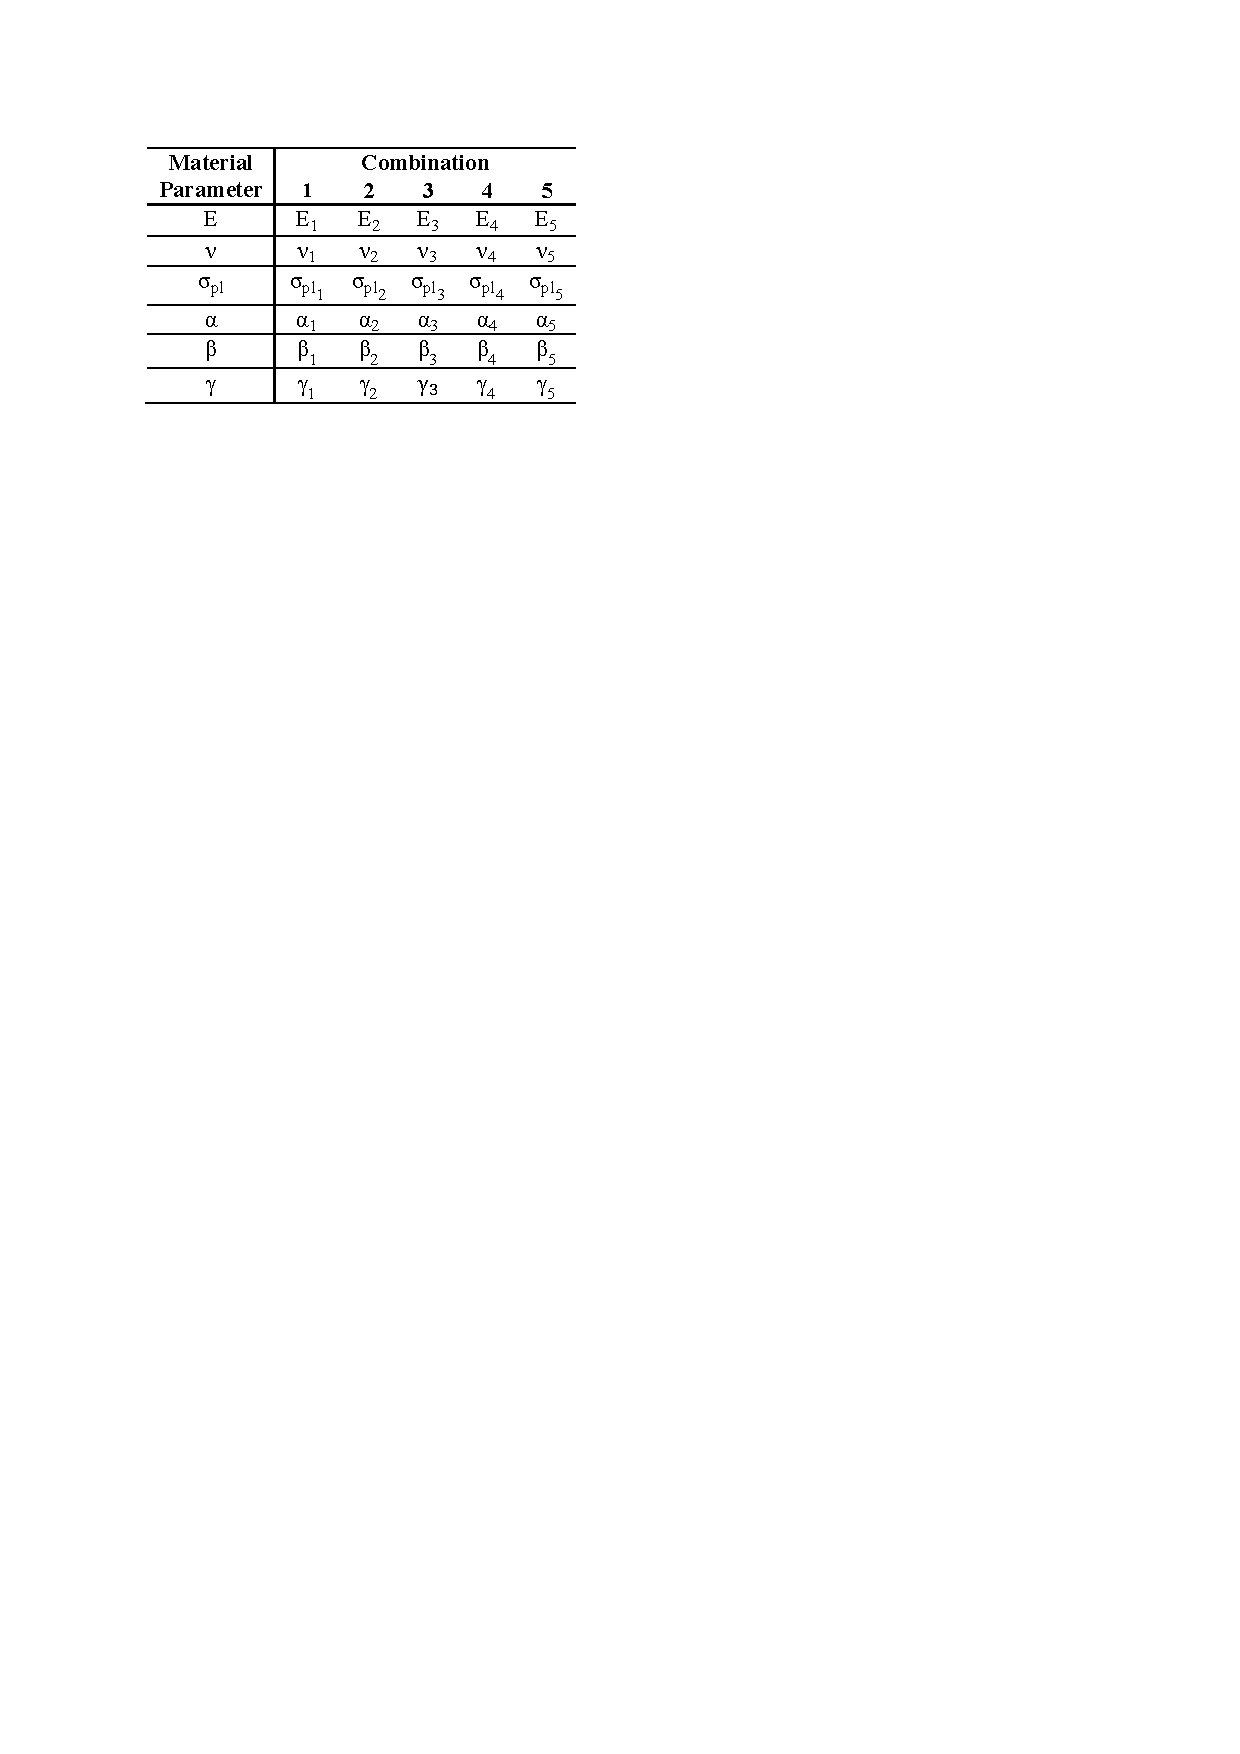
\includegraphics[width=1.0\textwidth]{initalValueComb.pdf}
                \vfill{}
		        \caption*{(a) Arrangement of initial value combination of material parameters}
                \label{tab:initialValueComb}
            \end{minipage}
            \hspace{0.05\textwidth} % Horizontal space between the minipage
            \begin{minipage}[T!][5.3cm][T!]{0.43\textwidth}
                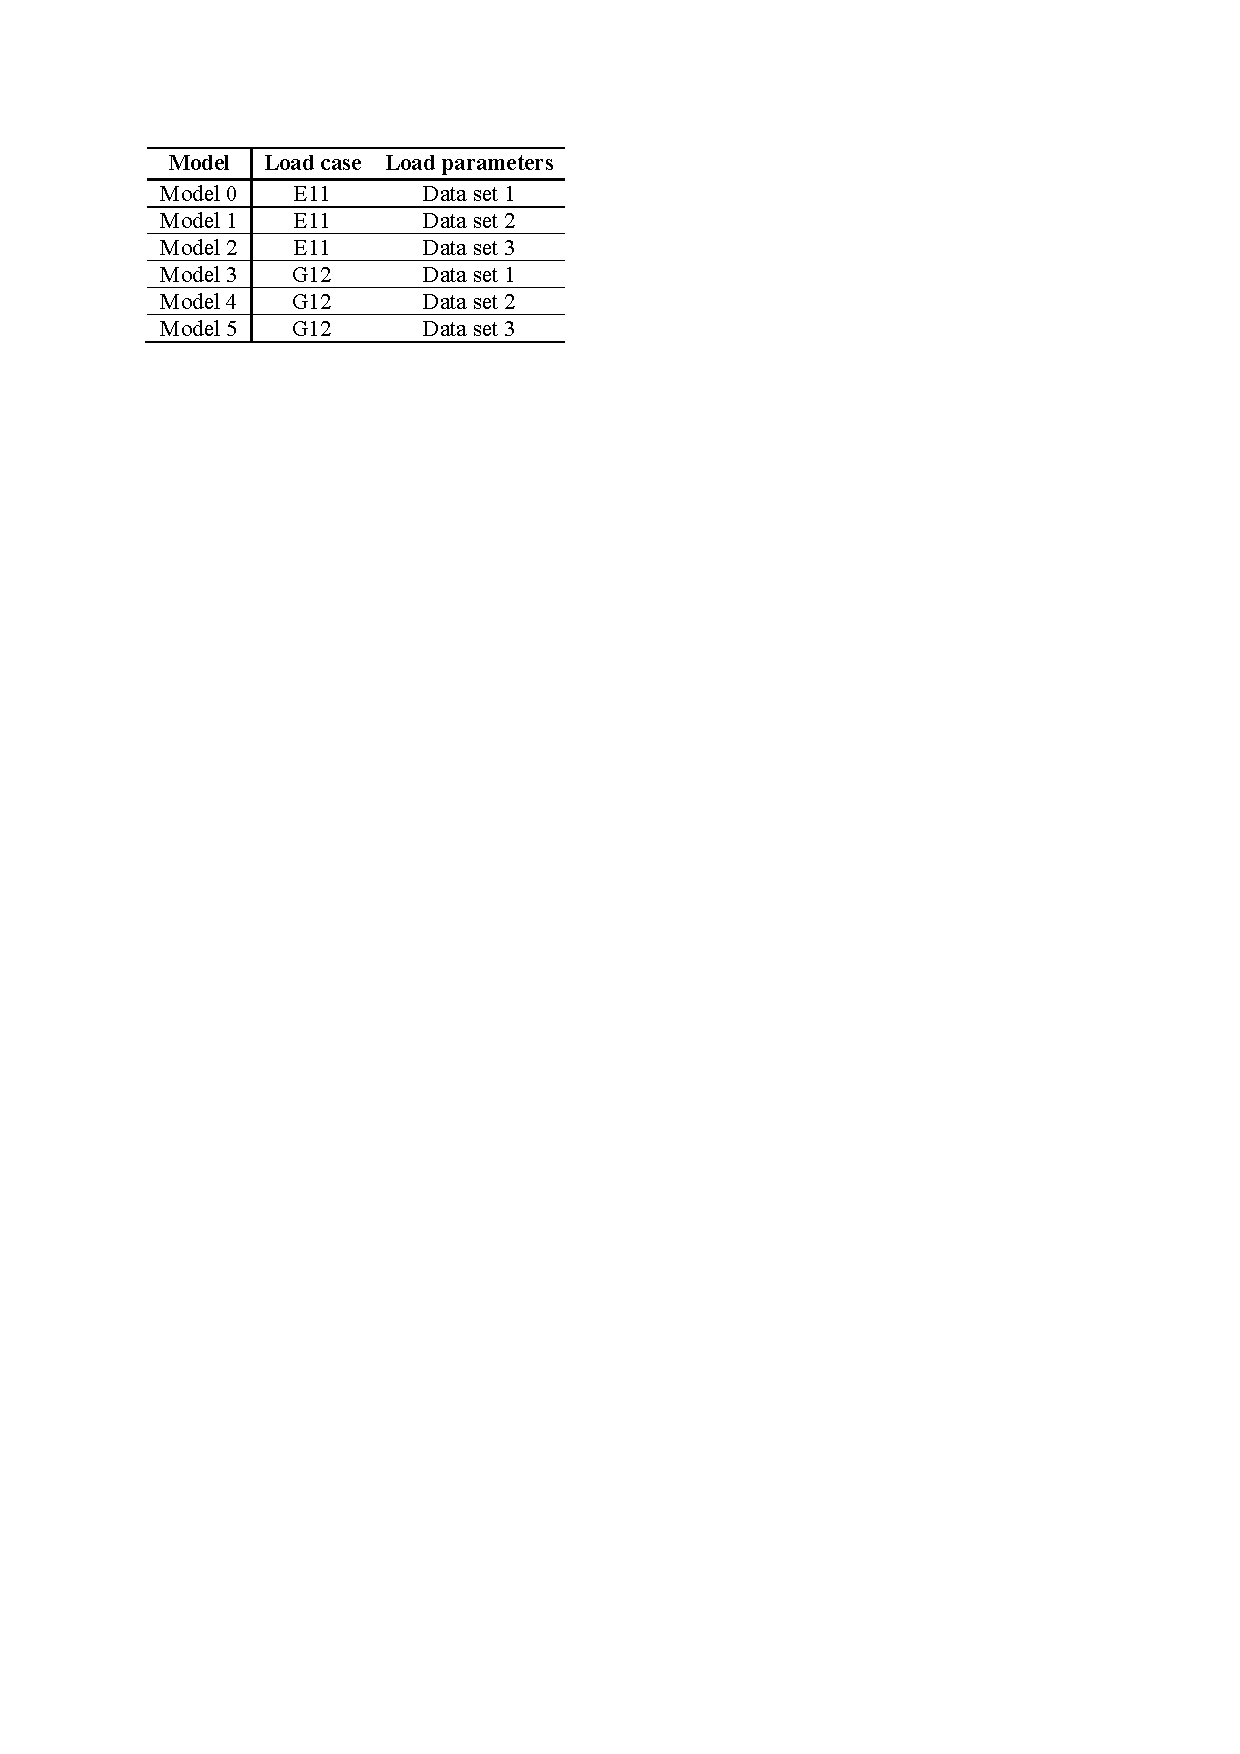
\includegraphics[width=1.0\textwidth]{ModelCombinations.pdf}
                \vfill{}
                \caption*{(b) Model creation for load case and parameter combinations}
                \label{tab:modelCombinations}
            \end{minipage}
        \end{minipage}    
        \caption{Loop conditions in preprocessing}
        \label{tab:ModelSettings}
	\end{table}
    
    Afterwards we start to construct the model. As discussed in section XX we use a cube with size 1x1x1 as model. We mesh the cube with 6x6x6 XXXX elements. The number of elements is a compromise between a coarse mesh for fast computation and a minimum number to avoid convergence errors. Although we use the hyperelastic material law in our optimization process, we first have to build the model with elastic material. This is necessary for the usage of easyPBC in the next step. Now we use the load case defined in the input file to create a easyPBC job to apply it on the cube. As discussed in chapter XXX we use easyPBC for the automatic construction of periodic boundary conditions. We use this set up to simulate a small detail of a infinitely large area (SCHLECHT FROMULIERT). Aside from that we use the generated boundary conditions for the applied load case. Since they act at a reference point a homogeneous load contribution is ensured. --> vlt auch in basics teil..
    However the settings from easyPBC contain some default values, we have to adjust. EasyPBC applies for every load case a uniform displacement with a standard fixed value. In our optimization we want to study cases with applied stresses as well. Additional we have to adapt the value of the load. For a correct comparison of the ABAQUS data with the MD-data we have to create evaluation points at similar load increments. In ABAQUS we can solve this issue by creating an amplitude. We register the evaluation points from the MD-data as steps and use this amplitude to apply the load. The value of the load is then set to 1 because it only defines the factor the amplitude is multiplied (see \autoref{fig:AbaqusSettings}). Afterwards we modify the increment settings. EasyPBC automatically creates increments with fixed size and without non-linear geometry effects. In order not to run into convergence errors we use automatic incrementation. Especially in the first load steps we observe large deformations. If we try to resolve such large deformations in one incrementation step ABAQUS cannot resolve the step. With automatic incrementation ABAQUS can adapt the number of increments per load step dynamically. The non-linear geometry effects have to be considered because of the material properties we use. As described before we build elastic material for the usage of easyPBC. In the following the code removes this material and substitutes it with a hyper-elastic material which is suitable for high non-linear deformation. By using this material, ABAQUS demands the inclusion of non-linear geometry effects. In the last step of preprocessing we store the model in a dictionary. We use this dictionary later to call the models for the optimization. We perform the preprocessing for all prescribed load cases. This means for example if we define E11, G12, and G23 as load cases, we create one model for each load case in the previous described manner. Furthermore, we loop over the load parameters and create separate models. In the end we have then for each combination of load case and load parameter one model. 

 

     \begin{figure}[H]
        \centering
        \begin{minipage}[T!]{1.0\textwidth}
            \centering
            \begin{minipage}[T!][9cm][T!]{0.35\textwidth}
                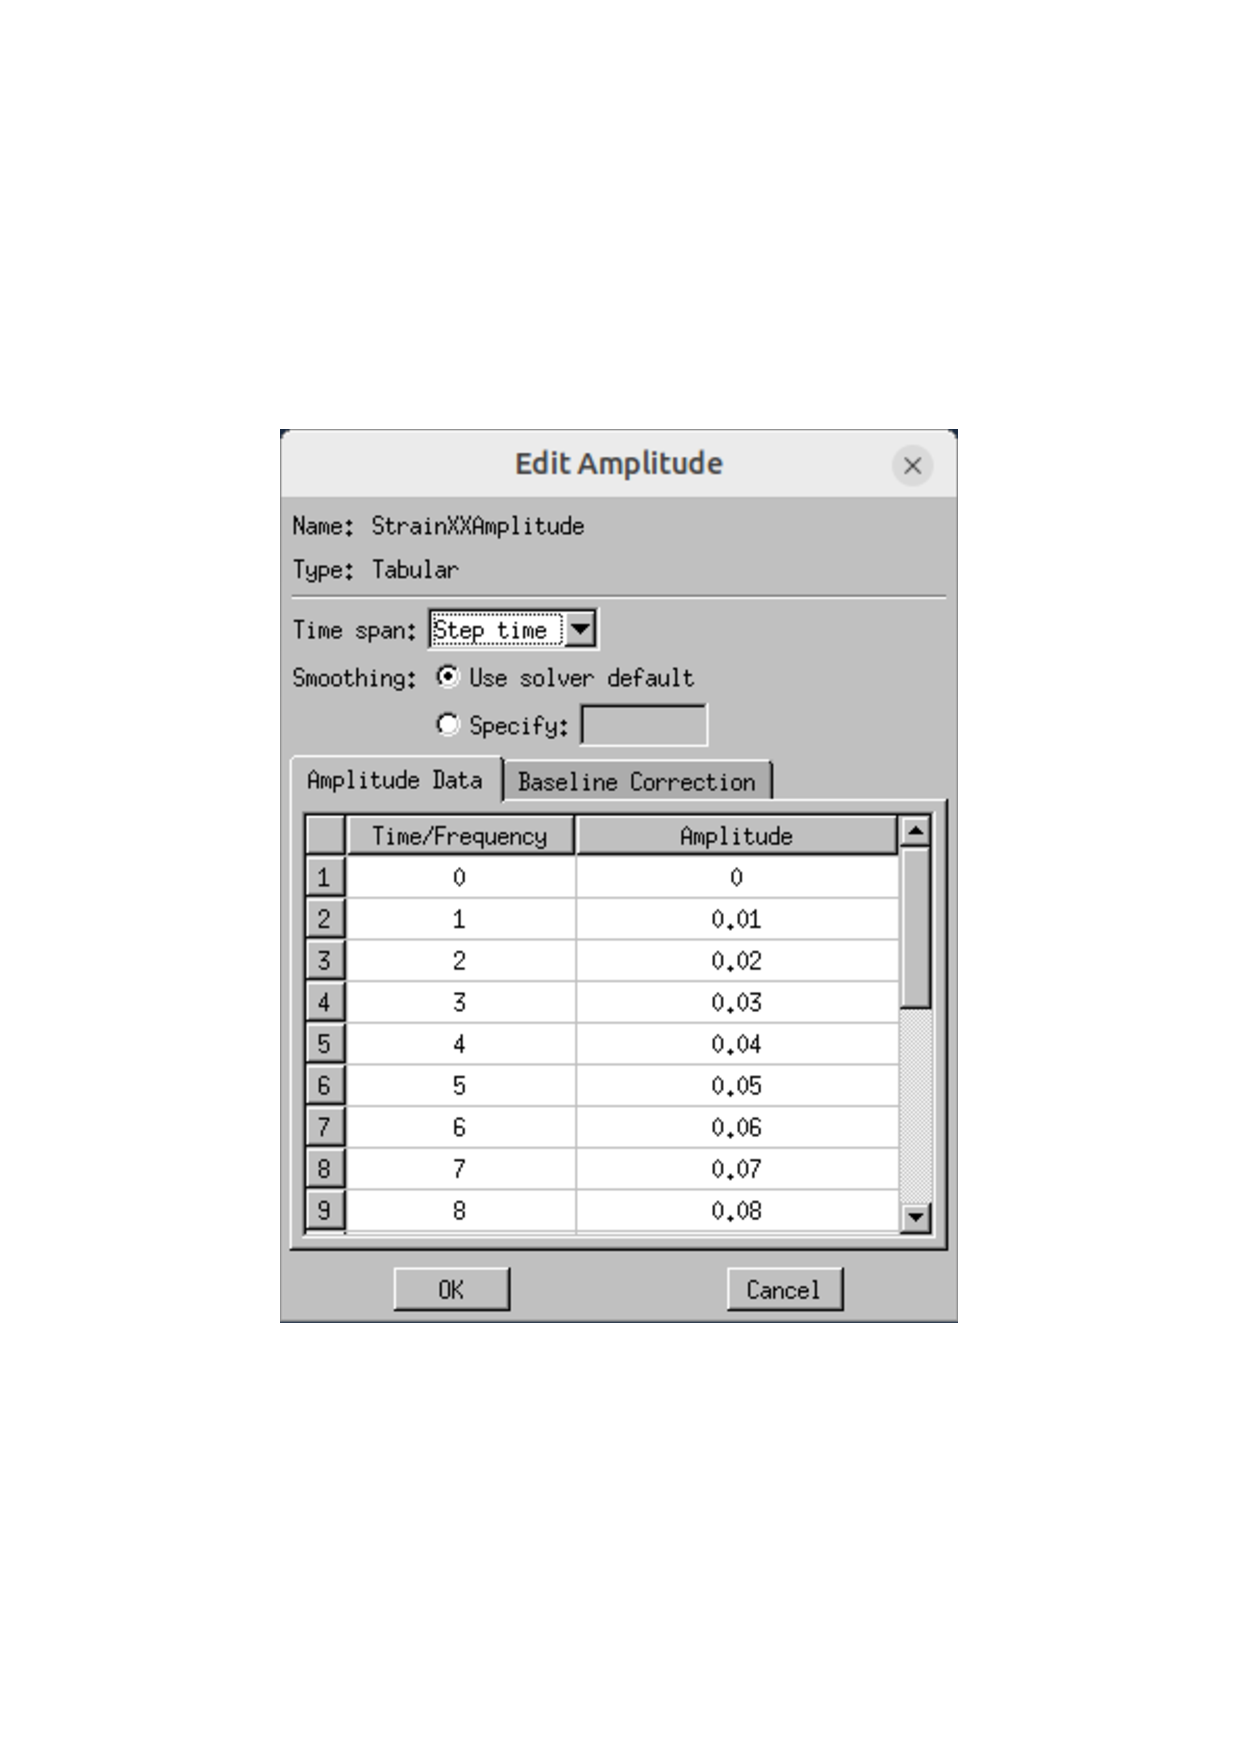
\includegraphics[width=1.0\textwidth]{Amplitude.pdf}
                \vfill{}
                \caption{Definition of load amplitude in ABAQUS}
                \label{fig:amplitudemenu}
            \end{minipage}
            \hspace{0.08\textwidth} % Horizontal space between the minipage
            \begin{minipage}[T!][9cm][T!]{0.35\textwidth}
                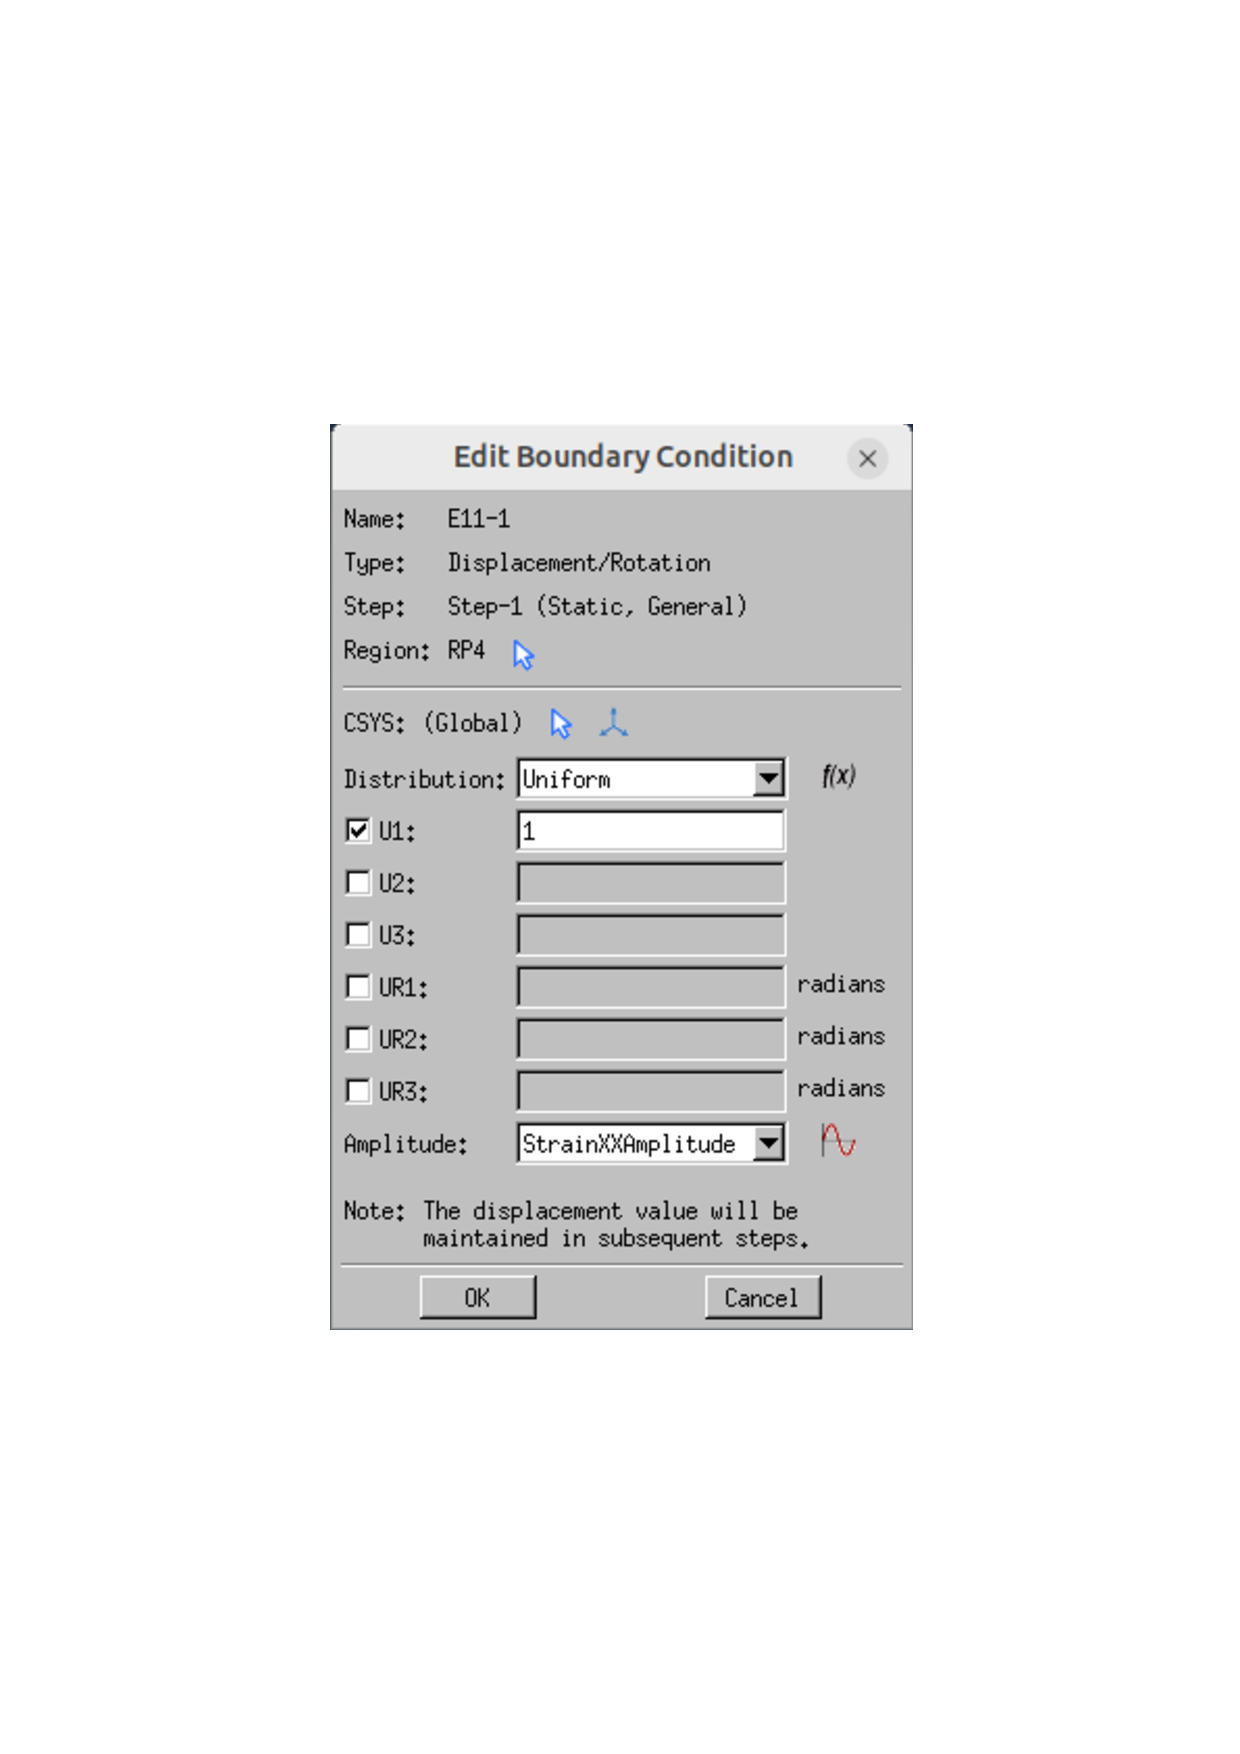
\includegraphics[width=1.0\textwidth]{BC.pdf}
                \vfill{}
                \caption{Boundary condition menu in ABAQUS}
                \label{fig:bcmenu}
            \end{minipage}
        \end{minipage}    
        \caption{Loop conditions in preprocessing}
        \label{fig:AbaqusSettings}
	\end{figure}
 
    \section{Optimisation process}

     \begin{table}[H]
		\centering
        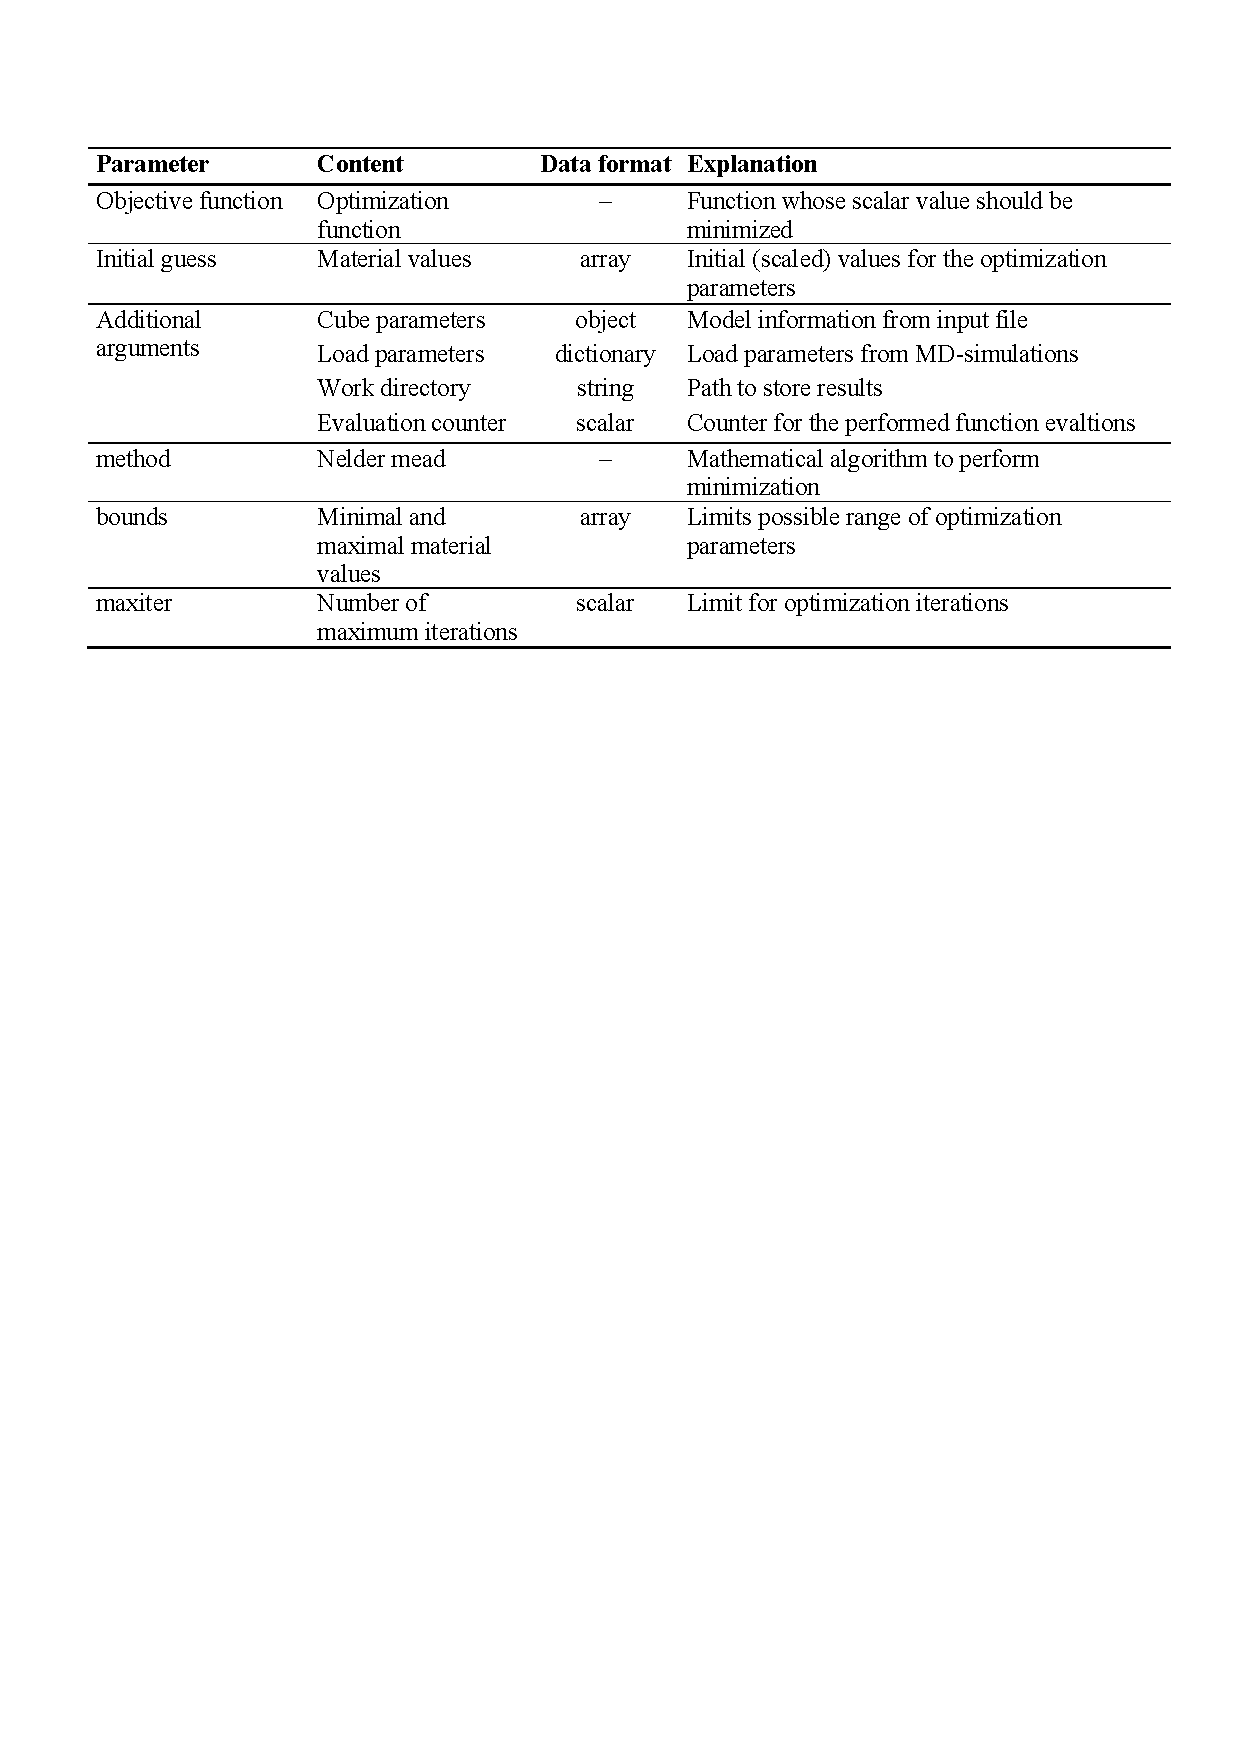
\includegraphics[width=0.95\textwidth]{minimizeFuncitonInput.pdf}
		\caption{Input parameters for SciPy minimize function}
		\label{tab:minimizeFunctionInput}
	\end{table}

    In the following section we describe the optimisation process. We start the processing by calling the scipy-minimize function. We pass this function various parameters to perform the optimization listed in table XX. (MEHR ÜBER INPUT PARAMETER INKL TABLEE ) The minimize function itself calls our self-written optimization function, where the evaluation takes place. As described before we create a model with a corresponding job for every combination of load case and load parameters and store them in a dictionary. Now we pass the whole dictionary to the optimization function. All of the models describe now different test cases for the same material. We want to use them all to get as much information as possible, such that we have to include all of them into the optimization process. To do so we have to calculate an error expression from all these analysis as described in section XX. 
    We start the process with rewriting the material values in all models. Since they all describe the same material we write the same values for every model. For the minimization computation optimization parameters are scaled in the bounds 0-1, that we have to rescale them first. Then we can use the rescaled parameters to compute the values for the plastic stress function with the formula for VOCE-hardening. Now we can update all material values. in the next step we handle the models successively. We start a job to perform the ABAQUS analysis and open the resulting output-data base. Afterwards we read the stresses from the odb. We do this by reading the fieldOutput variable 'S' and write the data in a stress directory. Since we need the stress-values at all the defined strain steps we read out every frame. One frame corresponds with one strain step. Additionally we loop over all directions (xx, yy, zz, xy, yz, xz). The same procedure is done for the strain values. Here it is important to read out the correct strain variable 'NE' (nominal strain). For hyperelastic materials ABAQUS uses as standard value the logarithmic strain ('LE'), which gives incorrect values in our studies. Then we store all values for all frames and directions in a dictionary again. Now we collected all required data to calculate the error. We do this in the way described in section XX. For a better structure of the code this part is outsourced in a separate function. We call this function and pass the stress and strain directory as well as the corresponding load parameters from the md-analysis. Then the computation runs and the function returns the rmse value for this job. Multiplied with its corresponding weights for load case and load parameters we add this value to the total error value. Now we restart the result reading and error computation for the next job. When all jobs are processed we have a total error value containing information from all jobs about the quality of the current material values. This value is the one we return our minimization function. It uses this values to compute internal the next material value combination to reduce the returned error value. Now one optimization iteration is performed. The new combination of material values is passed to our optimization function and it starts again. This process will run till our defined number of maximum iterations is reached. 

    \begin{enumerate}
        \item call scipy minimize with all necessary arguments
            1. function which shuold be minimized
            2. list with optimisation parameters
            3. additional arguments: data which are called in the minimized function:
                cubeparameter- object, mddaa dictionary, work directory, evaluation counter
            4. minimization method: nelder mead
            5. boundaries for optimization parameters
            6. options: return all (return function value from every iteration), maxiter (use max iteeration value as termination criterion)
    \end{enumerate}

    optimization function:
    \begin{enumerate}
        \item rescale material parameters
        \item compute plastic stresses
        \item delete elastic material
        \item write hyperelasitc material and update plastic material
        \item delete lock-files for job: they prevent the start of a job where a obd is already written
        \item list jobs in current work directory/ mdb
        \item iterate over jobs
        \item start job
        \item open odb
        \item create stress directory: for tensile load cases with normal direction, for shear load with shear direction
        \item loop over all directions
        \item loop over all frames from last step
        \item read fieldoutput 'S' from element set in current direction 
        \item write it in stress directory
        \item create strain directory
        \item loop over all directions
        \item loop over all frames from last step
        \item read fieldoutput 'NE' from element set in current direction 
        \item write it in strain directory
        \item call calculate rmse function
        \item call multiple save functions to store results
        \item when all jobs are finished: 
        \item multiple rmse from jobs with weights from parameter input (different weighting of load cases or md data sets)
        \item sum weighted rmse 
        \item save material parameters, rmse
        \item return total rmse

    \end{enumerate}

    
    
    calculate rmse function:

    \begin{itemize}
        \item loop over directions in stress directory if the direction should be anaylsed (parameter input)
        \item read out md data for this direction
        \item check if md data and odb data have the same length
        \item calculate squared differences for every step (array)
        \item weight array --> first data point is weighted with 100, because it is the only point in elastic domain 
        \item compute mean from array: sum over all weighted squared differences/ sum of all weights
        \item differentiate between tensile and shear load case:
            - use correlated weight 
        \item append to mse array
        \item same procedure  for strain directory
        \item sum up all mse values, divide by number of values (build mean value)
        \item wurzel ziehen
        \item return rmse
    \end{itemize}
        
    
    
    
    - formel wir sich RMSE zusamensetzt
    - welche schleifen gibt es?
    

    test cases:
    - linearere Zug
    - Zug und shear --> mit sinusform --> warum? 
    - cyclic tensile 
    